\chapter{性能测试与结果分析}

\section{实验环境配置}

本段将简单介绍运行Plasma的必要环境配置。这包括进行性能测试的集群硬件配置,以及编译、运行Plasma所需的其他软件要求。

\subsection{天河高性能集群硬件简介}

运行测试的天河高性能集群有超过100台CPU服务器,并由100GB的Infiniband高速网络连接而成。每个CPU节点的关键配置如下所示:

\begin{table}[h]
    \centering
    \caption{天河CPU服务器硬件配置}
    \begin{tabular}{*{4}{c}}
        \toprule
        硬件组件  & 数量 & 硬件型号 & 参数配置 \\
        \midrule
        CPU  	 & 2  & Intel(R) Xeon(R) Gold 6150 & \makecell{18核 @2.7GHz \\ L1 Cache 64K \\ L2 Cache 1024K \\ L3 Cache 25344K} \\
        \midrule
        内存 	 & 12 & / & \makecell{16Gb DDR4 \\ with ECC} \\
        \midrule
    	以太网卡 & 1  & Mellanox MT27710 Family [ConnectX-4 Lx]   & 25Gb/s \\
    	IB网卡   & 1  & Mellanox MT27700 Family [ConnectX-4] & 100Gb/s \\
        \bottomrule
    \end{tabular}
    \label{tab:hardware_config}
\end{table}

每个CPU服务器配备有双路Intel至强金牌处理器。每个CPU为6通道16G内存,因此每节点内存总量为192Gb。两路处理器形成两个NUMA节点,每节点上分别挂载有一张网卡。
该型服务器的硬件拓扑图如\autoref{fig:server_block}所示:

\begin{figure}[h]
	\centering
	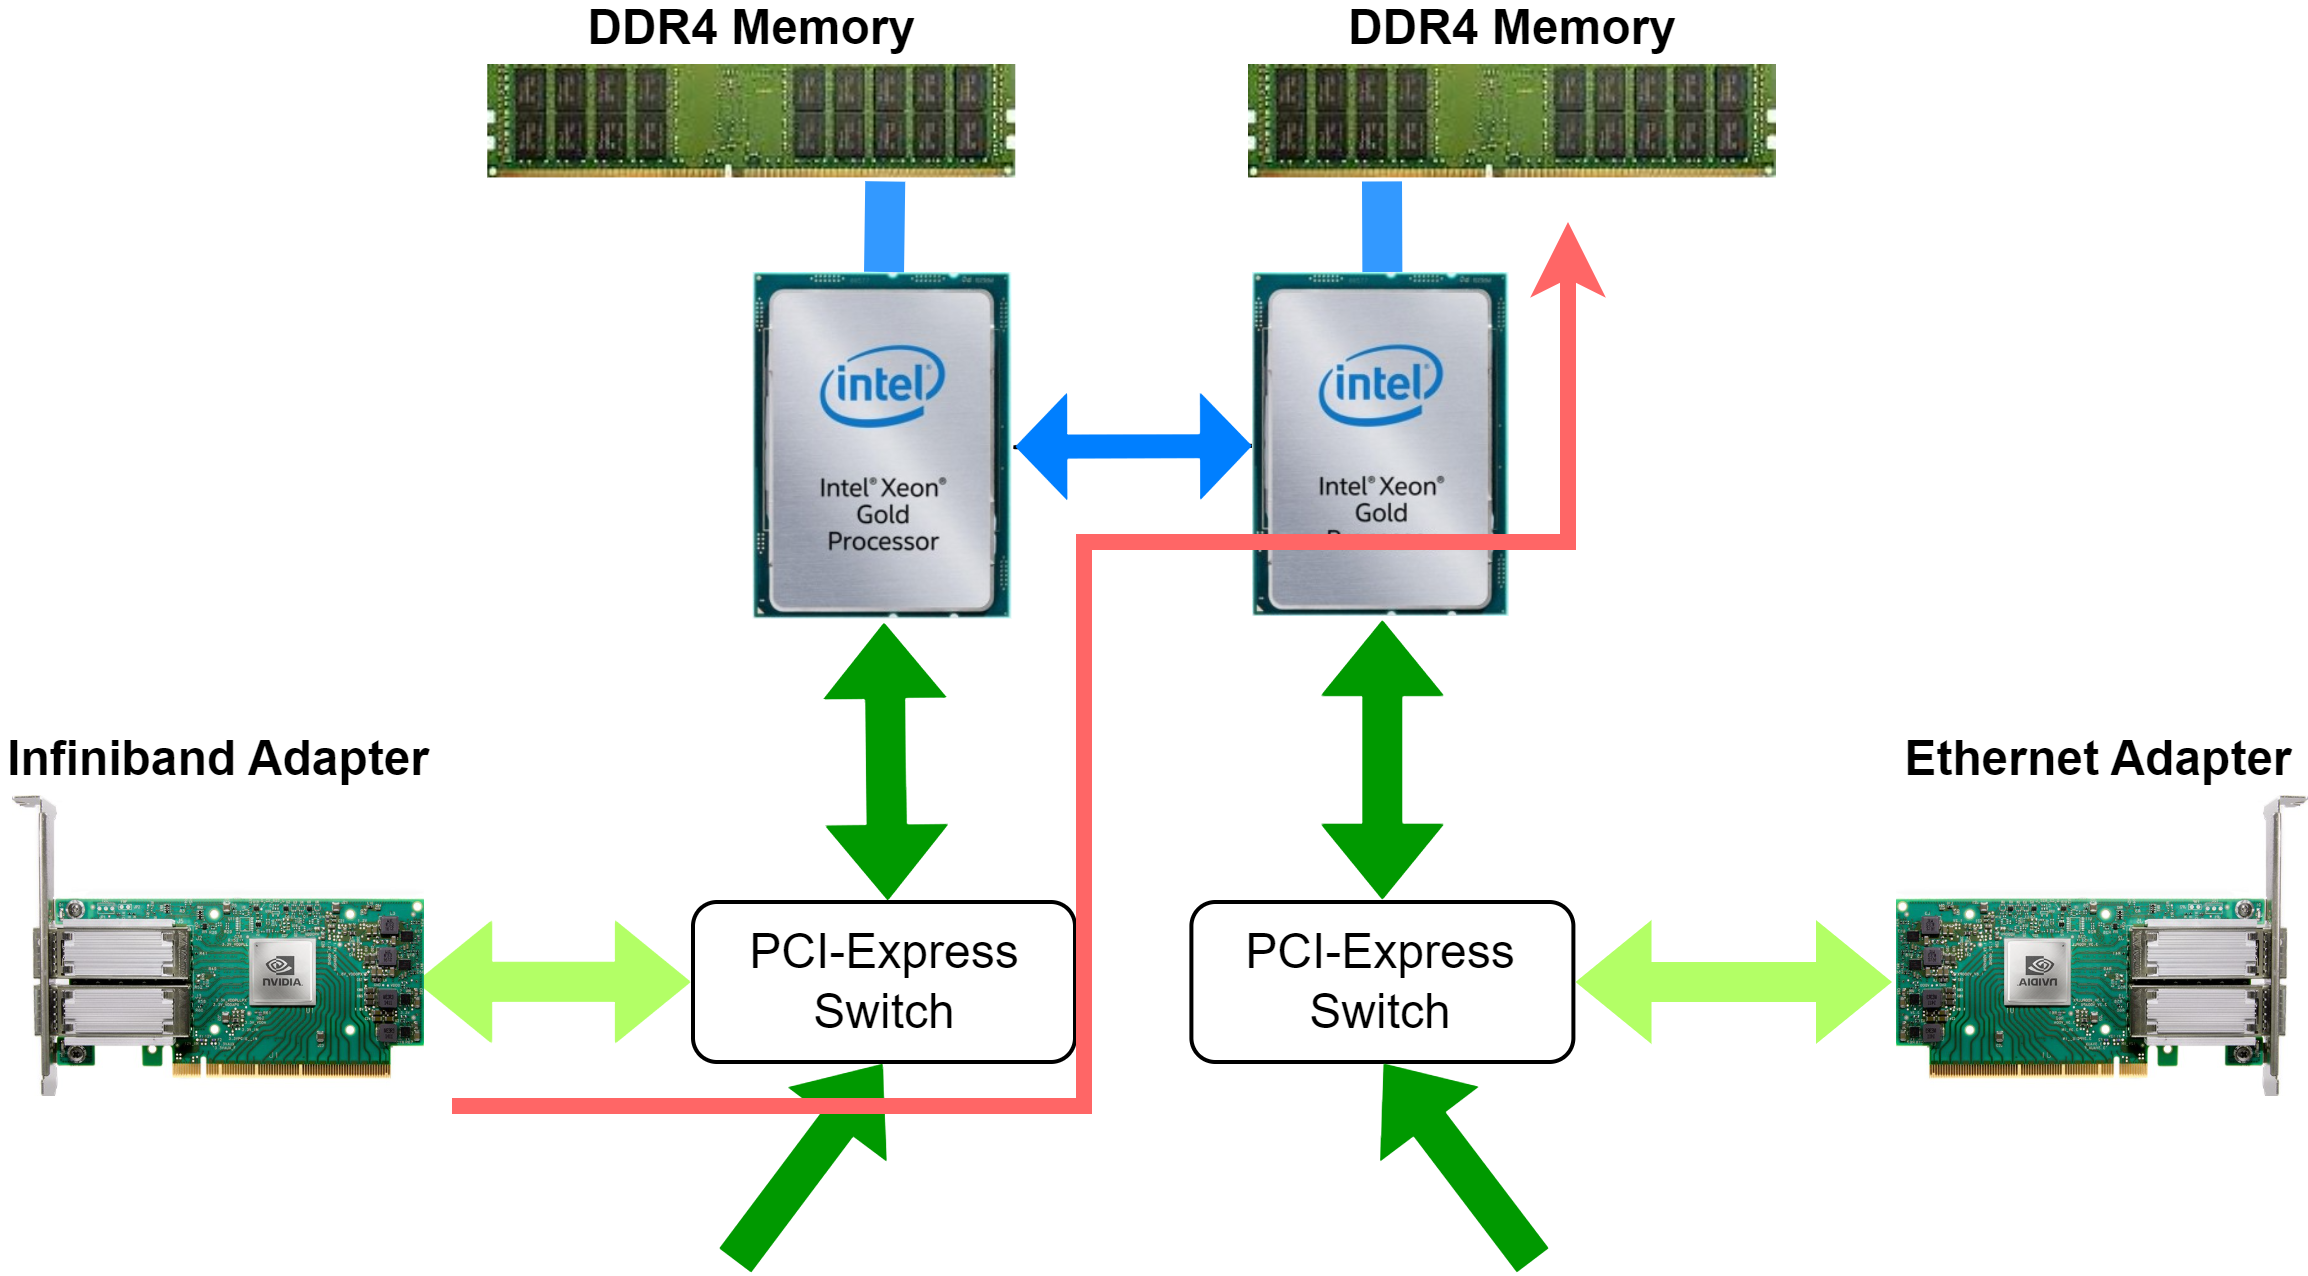
\includegraphics[width=0.7\textwidth]{image/chap04/server_block.png}
	\caption{天河CPU服务器硬件拓扑}
	\label{fig:server_block}
\end{figure}

需要注意的是,以太网卡和IB网卡分别挂在两个CPU的PCI-E Switch上,因而IB网卡只有在访问本NUMA节点的一半内存时拥有最佳性能——而访问远离它的CPU所控制的一半内存将会有
较大的性能损耗(\autoref{fig:server_block}中\textbf{红色访存路线})。这一特性对基于RDMA的网络通信性能有明显的影响,因此在实验中需要相应调整运行配置。

\subsection{软件环境简介}

\autoref{tab:software_config}展示了本章节各性能测试所运行的软件环境。操作系统一栏展示了天河高性能集群使用的Linux操作系统版本;软件依赖指的是成功编译出可正常执行
的Plasma程序所需要的前置软件;测试软件则表示为了编译基准测试程序、运行测试程序所需要的前置软件。软件名后的数字串分别表示这些软件的版本。

\begin{table}[h]
    \centering
    \caption{天河CPU服务器软件环境}
    \begin{tabular}{*{3}{c}}
        \toprule
        软件类型 & 软件名称  & 作用描述 \\
        \midrule
        操作系统 & CentOS Linux 7 & Linux内核版本3.10.0-957.el7.x86\_64 \\
        \midrule
        \multirow{3}{*}{软件依赖} & Redis@3.2.3 & \makecell{Redis服务器存放对象在Plasma集群的分布 \\ ae事件循环库驱动Plasma进程} \\
    	 & \makecell{uthash \\ utlist \\ utarray \\ utstring}@2.0.1 & \makecell{基于宏的C语言头文件库,\\ 包装了哈希表等高级数据结构} \\
		 & gcc@9.3.0 & 编译Redis和Plasma \\
        \midrule
    	\multirow{2}{*}{测试软件} & openmpi@4.1.1 & 编译基于MPI的多节点性能测试 \\
    	 & numactl@2.0.14 & 控制MPI进程在NUMA架构下的绑核运行 \\
        \bottomrule
    \end{tabular}
    \label{tab:software_config}
\end{table}

\section{NUMA架构对存储性能的影响}

\section{协议性能测试}

\section{结果分析}